\documentclass[12pt, a4paper]{report}

% Essential packages
\usepackage[utf8]{inputenc}
\usepackage[T1]{fontenc}
\usepackage{graphicx}
\usepackage{hyperref}
\usepackage[margin=2.5cm]{geometry}
\usepackage{listings}
\usepackage{xcolor}
\usepackage{float}
\usepackage{amsmath}
\usepackage{caption}
\usepackage{subcaption}
\usepackage{fancyhdr}
\usepackage{setspace}
\usepackage{tocloft}

% Set line spacing
\onehalfspacing

% Code listing settings
\definecolor{codegreen}{rgb}{0,0.6,0}
\definecolor{codegray}{rgb}{0.5,0.5,0.5}
\definecolor{codepurple}{rgb}{0.58,0,0.82}
\definecolor{backcolour}{rgb}{0.95,0.95,0.92}

% Define JSON language for listings
\lstdefinelanguage{json}{
    basicstyle=\normalfont\ttfamily,
    numbers=left,
    numberstyle=\scriptsize,
    stepnumber=1,
    numbersep=8pt,
    showstringspaces=false,
    breaklines=true,
    frame=lines,
    backgroundcolor=\color{backcolour},
    literate=
     *{0}{{{\color{numb}0}}}{1}
      {1}{{{\color{numb}1}}}{1}
      {2}{{{\color{numb}2}}}{1}
      {3}{{{\color{numb}3}}}{1}
      {4}{{{\color{numb}4}}}{1}
      {5}{{{\color{numb}5}}}{1}
      {6}{{{\color{numb}6}}}{1}
      {7}{{{\color{numb}7}}}{1}
      {8}{{{\color{numb}8}}}{1}
      {9}{{{\color{numb}9}}}{1}
      {:}{{{\color{punct}{:}}}}{1}
      {,}{{{\color{punct}{,}}}}{1}
      {\{}{{{\color{delim}{\{}}}}{1}
      {\}}{{{\color{delim}{\}}}}}{1}
      {[}{{{\color{delim}{[}}}}{1}
      {]}{{{\color{delim}{]}}}}{1},
}

\definecolor{numb}{rgb}{0.5,0,0.5}
\definecolor{delim}{rgb}{0.2,0.2,0.2}
\definecolor{punct}{rgb}{0.6,0.6,0.6}

\lstdefinestyle{mystyle}{
    backgroundcolor=\color{backcolour},   
    commentstyle=\color{codegreen},
    keywordstyle=\color{magenta},
    numberstyle=\tiny\color{codegray},
    stringstyle=\color{codepurple},
    basicstyle=\ttfamily\footnotesize,
    breakatwhitespace=false,         
    breaklines=true,                 
    captionpos=b,                    
    keepspaces=true,                 
    numbers=left,                    
    numbersep=5pt,                  
    showspaces=false,                
    showstringspaces=false,
    showtabs=false,                  
    tabsize=2
}
\lstset{style=mystyle}

% Page style
\pagestyle{fancy}
\fancyhf{}
\fancyhead[R]{\thepage}
\fancyhead[L]{\leftmark}
\renewcommand{\headrulewidth}{0.4pt}

% Document Info
\title{
    
\includegraphics[height=5cm]{assets/NNU_Logo.png} \\[1cm]
    
\includegraphics[height=2.5cm]{assets/Tinker_Blocks_Logo.png} \\[1cm]
    TinkerBlocks: Code, build, and drive! \\
    \large An Educational Tool for Teaching Programming Concepts Through Physical Blocks
}
\author{
    Amr Badran \\
    Izzat Alsharif
    \\\\
    \textbf{Supervisor:} Dr. Ashraf Armoush \\[0.5cm]
    \textbf{Department:} Computer Engineering \\
    \textbf{Faculty:} Engineering and Information Technology \\
    \textbf{University:} An-Najah National University
}
\date{June 10, 2025}

\begin{document}

% Front matter
\pagenumbering{roman}
\maketitle

% Certificate page
%\begin{center}
    \Large \textbf{CERTIFICATE}
    \end{center}
    
    \vspace{2cm}
    
    This is to certify that this project report entitled \textbf{"TinkerBlocks: Code, build, and drive! - An Educational Tool for Teaching Programming Concepts Through Physical Blocks"} by \textbf{Amr Badran} and \textbf{Izzat Alsharif}, submitted in partial fulfillment of the requirements for the degree of Bachelor of Technology in Computer Engineering of An-Najah National University, during the academic year 2024-25, is a bonafide record of work carried out under my guidance and supervision.
    
    The project demonstrates innovative approach to educational technology and represents significant contribution to the field of interactive learning systems.
    
    \vspace{3cm}
    
    \begin{center}
    \begin{tabular}{p{5cm} p{5cm}}
    & \\[2cm]
    \textbf{Dr. Ashraf Armoush} & \textbf{Head of Department} \\
    Project Supervisor & Computer Engineering Department \\
    Computer Engineering Department & An-Najah National University \\
    An-Najah National University & \\[1cm]
    Date: \_\_\_\_\_\_\_\_\_\_\_\_\_\_ & Date: \_\_\_\_\_\_\_\_\_\_\_\_\_\_ \\
    Place: Nablus, Palestine & Place: Nablus, Palestine \\
    \end{tabular}
    \end{center}
%\newpage

% Acknowledgment
\begin{center}
    \Large \textbf{ACKNOWLEDGMENT}
    \end{center}
    
    \vspace{1cm}
    
    We would like to express our sincere gratitude to our project supervisor \textbf{Dr. Ashraf Armoush} for his invaluable guidance, continuous support, and encouragement throughout this project. His expertise and insights have been instrumental in shaping this work and helping us overcome various technical challenges.
    
    We are grateful to the Computer Engineering Department at An-Najah National University for providing us with the necessary resources and facilities to complete this project successfully.
    
    We would also like to thank our families and friends for their unwavering support and patience during the development of this project. Their encouragement motivated us to push through difficult times and achieve our goals.

    Finally, we acknowledge all the researchers and educators whose work in the fields of educational technology, computer vision, and robotics inspired and informed our approach to this project.
    
    \vspace{2cm}
    
    \begin{flushright}
    Amr Badran \\
    Izzat Alsharif \\
    June 2025
    \end{flushright}
\newpage

% Abstract
\begin{center}
\Large \textbf{ABSTRACT}
\end{center}

\vspace{1cm}

TinkerBlocks is an educational tool designed to teach programming concepts to children through physical programming blocks and a programmable robotic car. The system combines physical learning with digital execution, allowing students to arrange physical blocks representing programming statements on a grid board to control a car that performs multiple tasks.

The project consists of three main components: a Raspberry Pi-based control system with multiple capabilities, a robotic car with advanced sensor integration, and a set of physical programming blocks. The Raspberry Pi performs image processing using OpenCV and EasyOCR to recognize block arrangements and instructions, interprets the visual programming language using an interpreter pattern, and controls the car through ESP32 communication.

The robotic car features differential steering with four DC motors, ultrasonic and IR sensors, an MPU-6050 gyroscope for precise movement and rotating, and a servo-controlled pen mechanism for drawing tasks.

Key technical achievements include the development of a good computer vision way for block recognition, implementation of an extensible command interpreter supporting loops, conditionals, and variables, creation of a reliable communication protocol between system components, and integration of multiple sensors for autonomous navigation and interaction detection.

This project successfully shows the feasibility of physical programming interfaces for educational purposes, providing an enjoyable way for children to learn programming concepts without the complexity of traditional text-based coding environments. Testing results show accurate block recognition, precise car movement control, and successful execution of complex programming logic including loops and conditional statements.

This project contributes to the growing field of educational robotics and physical programming, offering a scalable solution that can be adapted for various educational curricula and age groups.

\textbf{Keywords:} Educational Technology, Tangible Programming, Computer Vision, Robotics, Arduino, Raspberry Pi, Programming Education
\newpage

% Table of contents
\tableofcontents
\newpage

% List of figures
%\listoffigures
%\newpage

% List of tables
%\listoftables
%\newpage

% Main content - switch to arabic numbering
\pagenumbering{arabic}
\setcounter{page}{1}

% Chapters
\chapter{INTRODUCTION}

\section{Background and Motivation}

In an increasingly digital world, programming skills have become essential for students across all disciplines. However, traditional programming education often presents significant barriers for young learners. Abstract concepts, complex syntax, and screen-based interfaces can make programming feel disconnected from the physical world that children naturally explore and understand.

Educational technology has evolved to address these challenges, with hands-on learning approaches showing particular promise for engaging young minds. Physical manipulation and immediate visual feedback help children grasp abstract concepts more effectively than traditional lecture-based methods. This has led to growing interest in educational tools that bridge the gap between digital programming and physical interaction.

While various educational programming tools exist, most still rely on screen-based interfaces or require significant technical setup. There remains a need for intuitive systems that allow children to program through natural physical interaction while providing immediate, engaging feedback through real-world actions.

\section{Project Overview}

TinkerBlocks is an integrated educational system that transforms programming education through physical interaction. Children arrange programming blocks on a physical grid to control a robotic car, making programming concepts tangible and immediately visible through car movement and drawing.

The system consists of four main components working together:
\begin{itemize}
    \item Physical programming blocks representing commands, loops, and conditions
    \item Computer vision system that recognizes block arrangements in real-time
    \item Intelligent robotic car that executes programs with sensor feedback
    \item Mobile application for more engaging features
\end{itemize}

This integration creates a complete learning environment where children can progress from simple movement commands to complex algorithms involving variables, loops, and sensor-based decision making.

\section{Problem Statement}

Current programming education tools for children face several key challenges:

\begin{enumerate}
    \item \textbf{Abstract Learning Environment}: Programming concepts remain disconnected from physical reality, making them difficult for young learners to grasp
    \item \textbf{Limited Immediate Feedback}: Most tools provide only visual feedback on screens rather than real-world interaction
    \item \textbf{Complex Setup Requirements}: Many educational robotics solutions require significant technical knowledge to operate
    \item \textbf{Fragmented Learning Experience}: Existing tools often focus on single aspects (either programming OR robotics) rather than integrated learning
    \item \textbf{Scalability Issues}: Most solutions are designed for individual use rather than classroom environments
\end{enumerate}

\section{Proposed Solution}

TinkerBlocks addresses these challenges through an innovative approach that combines multiple technologies into a cohesive educational experience:

\textbf{Physical Programming Interface}: Children arrange blocks representing programming commands on a grid, making abstract concepts concrete and manipulable.

\textbf{Real-time Computer Vision}: Advanced image processing recognizes block arrangements and translates them into executable programs without requiring manual input.

\textbf{Intelligent Robotic Execution}: A sophisticated car equipped with sensors executes programs while providing immediate visual feedback through movement and drawing capabilities.

\textbf{Integrated System Architecture}: All components communicate seamlessly, creating a unified experience from block placement to program execution.

This approach allows children to learn programming concepts naturally through physical manipulation while seeing immediate results in the real world.

\section{Objectives}

The primary objectives of this project are:

\subsection{Educational Objectives}
\begin{enumerate}
    \item Create an intuitive programming interface accessible to children without prior technical knowledge
    \item Provide immediate visual feedback to reinforce learning of programming concepts
    \item Support progressive learning from basic commands to advanced programming constructs
    \item Enable collaborative programming activities in classroom settings
\end{enumerate}

\subsection{Technical Objectives}
\begin{enumerate}
    \item Develop accurate computer vision algorithms for real-time block recognition
    \item Implement robust communication between multiple system components
    \item Create a comprehensive command interpreter supporting loops, conditionals, and variables
    \item Design reliable robotic hardware capable of precise movement and sensor integration
\end{enumerate}

\section{Scope and Contributions}

\subsection{Project Scope}
This project delivers a complete working system including:
\begin{itemize}
    \item Hardware design and construction of the robotic car with sensor integration
    \item Computer vision pipeline for block recognition and grid mapping
    \item Command interpreter supporting complex programming constructs
    \item Mobile application for more engaging features
    \item Integration protocols enabling seamless communication between all components
    \item Testing and validation in real-world educational scenarios
\end{itemize}

\subsection{Key Contributions}
\begin{itemize}
    \item Integration of computer vision, robotics, and mobile technology for educational purposes
    \item Development of an accessible physical programming interface for young learners
    \item Creation of a scalable system architecture suitable for classroom deployment
    \item Demonstration of effective tangible programming for computational thinking education
\end{itemize}

\section{Report Structure}

This report documents the complete development and implementation of the TinkerBlocks system:

\textbf{Chapter 2} reviews existing educational technology and programming tools, positioning TinkerBlocks within the current landscape of educational robotics.

\textbf{Chapter 3} presents the system architecture and design decisions, including hardware specifications, software architecture, and integration strategies.

\textbf{Chapter 4} details the implementation of all system components, from computer vision algorithms to robotic control systems.

\textbf{Chapter 5} concludes with project achievements, educational impact, and recommendations for future development.

Appendices provide technical documentation, code examples, and detailed system specifications for implementation reference.
\chapter{LITERATURE REVIEW}

\section{Educational Robotics}

Educational robotics has shown as a powerful tool for teaching STEM concepts, particularly programming and computational thinking. The field has evolved significantly since the introduction of Logo and the turtle graphics system in the 1960s, which first demonstrated the potential of robotics in education.

Modern educational robotics platforms like LEGO Mindstorms, VEX Robotics, and Arduino-based systems have made robotics more accessible to students and educators. These platforms typically combine programmable microcontrollers with sensors, actuators, and mechanical components, allowing students to build and program their own robots.

Research has shown that educational robotics can improve student thinking, problem-solving skills, and understanding of programming concepts. The immediate visual and touchable feedback provided by robotic systems helps students understand abstract programming concepts and debug their code more effectively.

\section{Tangible Programming Interfaces}

Tangible programming interfaces represent a paradigm shift from traditional screen-based programming environments to physical manipulation of programming constructs. This approach is rooted in the theory of embodied cognition, which suggests that physical interaction with objects enhances learning and understanding.

\subsection{Historical Development}

The concept of tangible programming can be traced back to early educational toys like the Big Trak programmable robot and more recent systems like the AlgoBlock system developed at MIT. These early systems demonstrated that children could understand programming concepts through physical manipulation long before they could master text-based programming languages.

\subsection{Current Approaches}

Several systems have explored tangible programming interfaces:

\begin{itemize}
    \item \textbf{Cubetto}: A wooden robot that uses colored blocks to represent programming commands
    \item \textbf{Code \& Go}: A board game approach to teaching programming logic
    \item \textbf{Osmo Coding}: Uses physical blocks detected by tablet cameras
    \item \textbf{KIBO}: A construction kit for children to build and program robots using wooden blocks
\end{itemize}

\subsection{Advantages and Challenges}

Tangible programming interfaces offer several advantages:
\begin{itemize}
    \item Reduced cognitive load by eliminating syntax requirements
    \item Enhanced spatial understanding of program flow
    \item Support for collaborative programming activities
    \item Accessibility for learners with different abilities
\end{itemize}

However, they also present challenges:
\begin{itemize}
    \item Limited scalability for complex programs
    \item Physical constraints on program size
    \item Recognition accuracy in computer vision-based systems
    \item Higher hardware costs compared to software-only solutions
\end{itemize}

\section{Computer Vision in Educational Applications}

Computer vision has become increasingly important in educational technology, enabling systems to interpret and respond to physical student interactions. In the context of tangible programming interfaces, computer vision serves as the bridge between physical manipulation and digital execution.


\subsection{Constructivist Learning Theory}

Based on the work of Jean Piaget and Seymour Papert, constructivist learning theory emphasizes learning through construction and experimentation. This theory has been particularly influential in the design of programming tools for children, promoting hands-on exploration over direct instruction.

\subsection{Block-Based Programming Languages}

Visual programming languages like Scratch, Blockly, and Alice have revolutionized programming education by providing drag-and-drop interfaces that eliminate syntax errors and focus on logic and computational thinking. These tools have demonstrated the effectiveness of visual approaches to programming education.

\subsection{Computational Thinking}

Computational thinking encompasses four key skills:
\begin{itemize}
    \item \textbf{Decomposition}: Breaking complex problems into smaller parts
    \item \textbf{Pattern Recognition}: Identifying similarities and patterns
    \item \textbf{Abstraction}: Focusing on essential features while ignoring irrelevant details
    \item \textbf{Algorithm Design}: Creating step-by-step solutions
\end{itemize}

Effective programming education tools should support the development of these skills through appropriate progression.

\section{Related Systems and Technologies}

\subsection{Commercial Educational Robotics Platforms}

Several commercial platforms share similarities with TinkerBlocks:

\textbf{LEGO Mindstorms:} A comprehensive robotics platform that combines programmable bricks with sensors and motors. While highly capable, it relies on screen-based programming interfaces and requires significant investment in components.

\textbf{Bee-Bot and Blue-Bot:} Simple programmable robots designed for early childhood education. These systems use button-based programming but lack the flexibility of a visual programming interface.

\textbf{Dash and Dot:} Smartphone-controlled robots with visual programming apps. While accessible, they depend on mobile devices and don't provide tangible programming experiences.

\subsection{Research Prototypes}

Academic research has produced several innovative approaches to tangible programming:

\textbf{Tern:} A tangible programming system that uses physical tiles arranged on a surface, detected by an overhead camera. This system demonstrated the feasibility of camera-based block recognition.

\textbf{Topobo:} A 3D construction kit with kinetic memory, allowing children to teach robots behaviors through physical demonstration.

\textbf{FlowBlocks:} A tangible programming system for controlling robotic devices using magnetic blocks that can be arranged on a whiteboard.

\section{Gaps in Current Research}

Despite significant progress in educational robotics and tangible programming interfaces, several gaps remain:

\begin{enumerate}
    \item \textbf{Limited Integration:} Most systems focus on either robotics or programming, but few successfully integrate both in a easy learning experience.
    
    \item \textbf{Scalability Issues:} Many tangible programming systems are limited in the complexity of programs they can represent.
    
    \item \textbf{Curriculum Integration:} Most systems exist as standalone tools rather than integrated components of educational curricula.
    
    \item \textbf{Accessibility:} Limited research has been conducted on making these systems accessible to learners with different abilities and learning styles.
\end{enumerate}

\section{Positioning of TinkerBlocks}

TinkerBlocks addresses several of these gaps by:

\begin{itemize}
    \item Providing seamless integration between tangible programming and robotic execution
    \item Supporting multiple game modes that aims to different learning objectives
    \item Using modern computer vision techniques for robust block recognition
    \item Implementing a scalable interpreter architecture that can support complex programming constructs
    \item Designing a modular system that can be extended and adapted for different educational contexts
\end{itemize}

The system builds upon the strengths of existing approaches while addressing their limitations through innovative technical solutions and design decisions.
\chapter{SYSTEM DESIGN AND ARCHITECTURE}

\section{System Overview}

TinkerBlocks is a comprehensive educational system that integrates multiple hardware and software components to create a seamless tangible programming experience. The system architecture follows a modular design approach, ensuring scalability, maintainability, and extensibility.

The system consists of four main components:
\begin{enumerate}
    \item \textbf{Programming Grid}: Physical board with camera for block recognition
    \item \textbf{Raspberry Pi Control System}: Central processing unit for computer vision and control
    \item \textbf{Robotic Car}: Programmable vehicle with sensors and actuators
    \item \textbf{Programming Blocks}: Physical blocks representing programming constructs
\end{enumerate}

\section{System Architecture}

The TinkerBlocks architecture consists of a three-layer design pattern:

\subsection{Core Layer}
The core layer provides foundational infrastructure with zero dependencies on other modules:
\begin{itemize}
    \item WebSocket server for real-time communication
    \item Process controller for workflow management
    \item Centralized configuration management
    \item Generic workflow execution framework
\end{itemize}

\subsection{Vision Layer}
The vision layer handles all computer vision and image processing tasks:
\begin{itemize}
    \item Image capture from camera systems
    \item Grid detection with perspective transformation
    \item OCR processing for text extraction
    \item Mapping of detected text to grid positions
\end{itemize}

\subsection{Engine Layer}
The engine layer implements the command interpreter and execution system:
\begin{itemize}
    \item Command parsing and validation
    \item Program execution with state management
    \item Variable and expression evaluation
    \item Control flow implementation (loops, conditionals)
\end{itemize}

\begin{figure}[H]
    \centering
    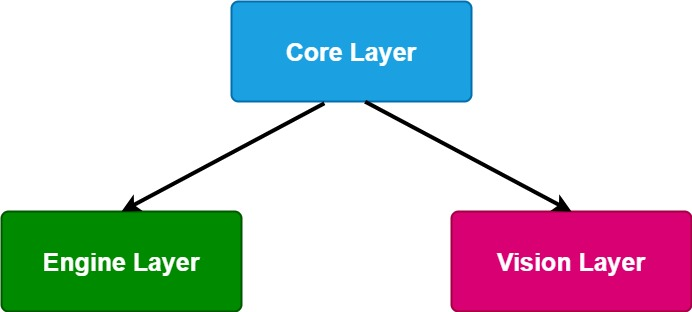
\includegraphics[width=0.8\textwidth]{assets/System_Arch.jpg}
    \caption{System Architecture}
    \label{fig:system_architecture}
\end{figure}

\section{Hardware Design}

\subsection{Robotic Car Specifications}

The robotic car serves as the primary execution platform for student programs. The design ensures precision, reliability, and educational value.

\subsubsection{Mechanical Design}
\begin{itemize}
    \item \textbf{Chassis}: Custom wooden frame (10cm × 20cm)
    \item \textbf{Propulsion}: Four DC motors with differential steering
    \item \textbf{Weight}: Approximately 500g 
    \item \textbf{Wheel Configuration}: Four-wheel drive
\end{itemize}

\subsubsection{Control Electronics}
\begin{itemize}
    \item \textbf{Main Controller}: Arduino Mega 2560 (primary control and sensor management)
    \item \textbf{WiFi Module}: ESP32 (wireless communication and API bridge)
    \item \textbf{Motor Drivers}: Two H-bridge modules for motor control
    \item \textbf{Power Management}: Voltage regulator (11.1V to 5V conversion)
\end{itemize}

\subsubsection{Sensor Integration}
\begin{itemize}
    \item \textbf{Navigation}: MPU-6050 gyroscope and accelerometer for precise orientation
    \item \textbf{Obstacle Detection}: HC-SR04 ultrasonic sensor (front-mounted)
    \item \textbf{Line Detection}: Two IR sensors for path boundary detection
    \item \textbf{Drawing Mechanism}: Servo-controlled pen for drawing operations
\end{itemize}

\subsubsection{Power System}
\begin{itemize}
    \item \textbf{Battery Pack}: Three 3.7V lithium-ion batteries (11.1V total)
    \item \textbf{Operating Time}: Approximately 2-3 hours of continuous operation
    \item \textbf{Charging}: External charging system with safety protection
\end{itemize}

\subsection{Programming Grid Board}

The programming grid serves as the interface for arranging programming blocks and capturing their configuration.

\subsubsection{Physical Structure}
\begin{itemize}
    \item \textbf{Grid Size}: 16 columns × 10 rows (configurable)
    \item \textbf{Block Placement}:  drag and drop by hand into holes.
    \item \textbf{Material}: wood construction (PVC)
    \item \textbf{Portability}: Lightweight design for classroom use
\end{itemize}

\subsubsection{Camera System (OAK-D)}
\begin{itemize}
    \item \textbf{Position}: Overhead mounting for full grid visibility
    \item \textbf{Resolution}: High-resolution camera for accurate text recognition
    \item \textbf{Lighting}: Controlled lighting conditions for consistent image quality
    \item \textbf{Calibration}: Automated corner detection and perspective correction
\end{itemize}

\subsection{Control Station}

The Raspberry Pi-based control station manages the entire system operation.

\subsubsection{Hardware Specifications}
\begin{itemize}
    \item \textbf{Processor}: Raspberry Pi 4 (2GB RAM)
    \item \textbf{Storage}: 32GB microSD card for system and data storage
    \item \textbf{Display}: Tablet for status and game mode information
    \item \textbf{Input}: Buttons and Applcation on Tablet for user interaction
    \item \textbf{Connectivity}: WiFi for car communication, USB for camera
\end{itemize}

\section{Software Architecture}

\subsection{Modular Design Principles}

The software architecture follows clean architecture principles with clear separation of concerns:

\begin{itemize}
    \item \textbf{Dependency Inversion}: Core modules have zero dependencies on implementation details
    \item \textbf{Protocol-Based Design}: Interfaces defined through Python protocols for extensibility
    \item \textbf{Async-First Architecture}: Built on asyncio for concurrent operations
    \item \textbf{Workflow Pattern}: Generic execution framework supporting cancellation and chaining
\end{itemize}

\subsection{Communication Architecture}

The system implements a multi-protocol communication architecture:

\subsubsection{WebSocket Communication}
\begin{itemize}
    \item Real-time bidirectional communication between components
    \item JSON-based message protocol for command and status exchange
    \item Broadcast support for multiple client connections
    \item Connection management with automatic reconnection
\end{itemize}

\subsubsection{Serial Communication}
\begin{itemize}
    \item Arduino-ESP32 communication via UART (115200 baud)
    \item Command-response protocol with JSON payloads
    \item Error handling and timeout management
    \item Flow control for reliable data transmission
\end{itemize}

\subsubsection{HTTP API}
\begin{itemize}
    \item RESTful API exposed by ESP32 for car control
    \item Stateless design for reliable remote operation
    \item JSON request/response format for all endpoints
    \item Error reporting with appropriate HTTP status codes
\end{itemize}

\section{Programming Language Design}

\subsection{Visual Programming Constructs}

The TinkerBlocks programming language supports fundamental programming concepts through physical blocks:

\subsubsection{Movement Commands}
\begin{itemize}
    \item \textbf{MOVE}: Forward/backward movement with distance parameters
    \item \textbf{TURN}: Left/right rotation with angle specifications
    \item \textbf{WAIT}: Pause execution for specified time duration
\end{itemize}

\subsubsection{Control Flow}
\begin{itemize}
    \item \textbf{LOOP}: Repetition with count or conditional parameters
    \item \textbf{IF/ELSE}: Conditional execution based on sensor inputs
    \item \textbf{WHILE}: Conditional loops with real-time evaluation
\end{itemize}

\subsubsection{Data Manipulation}
\begin{itemize}
    \item \textbf{SET}: Variable assignment and arithmetic operations
    \item \textbf{Variables}: Named storage for numeric and boolean values
    \item \textbf{Expressions}: Mathematical and logical operations
\end{itemize}

\subsubsection{Input/Output}
\begin{itemize}
    \item \textbf{PEN\_UP/PEN\_DOWN}: Drawing control for creative tasks
    \item \textbf{Sensor Values}: Distance, obstacle detection, line sensing
    \item \textbf{Boolean Operations}: Logical combinations of conditions
\end{itemize}

\subsection{Syntax and Semantics}

The visual programming language uses indentation-based syntax similar to Python:

\begin{itemize}
    \item \textbf{Block Arrangement}: Left-to-right, top-to-bottom reading order
    \item \textbf{Indentation}: Column position determines nesting level

\end{itemize}



\section{User Interface Design}

\subsection{Physical Interface}

The system provides intuitive physical interaction through:

\begin{itemize}
    \item \textbf{Block Placement}: mechanical guides for precise positioning
    \item \textbf{Visual Feedback}: Real-Time updates sending to an app.
    \item \textbf{Control Buttons}: Start, stop buttons
    \item \textbf{Display Screen}: a Mobile Screen with App running on it.
\end{itemize}

\subsection{Digital Interface}

\subsubsection{Monitoring}
\begin{itemize}
    \item camera feed showing current block arrangement
    \item Program execution visualization with updates sending to app
\end{itemize}

\subsubsection{Educational Features}
\begin{itemize}
    \item Step-by-step program execution with optional pauses
    \item Error messages with educational explanations
\end{itemize}

\section{Scalability and Extensibility}

\subsection{Hardware Scalability}

The modular hardware design supports future extensions:

\begin{itemize}
    \item \textbf{Additional Sensors}: Expandable I/O for new sensor types
    \item \textbf{Multiple Cars}: Support for multi-robot scenarios
    \item \textbf{Larger Grids}: Scalable grid sizes for complex programs
    \item \textbf{Enhanced Actuators}: Additional output devices (speakers, lights)
\end{itemize}

\subsection{Software Extensibility}

The software architecture enables easy extension:

\begin{itemize}
    \item \textbf{Command Registry}: Plugin-style command addition
    \item \textbf{Workflow Framework}: Generic execution patterns
    \item \textbf{Protocol Abstraction}: Support for different communication methods
    \item \textbf{ِAI}: Support for AI coding like Github-copilot
\end{itemize}

\section{Performance Requirements}

\subsection{Real-time Performance}

The system is designed to meet specific performance criteria:

\begin{itemize}
    \item \textbf{Image Processing}: Block recognition within 2 seconds
    \item \textbf{Program Execution}: Immediate response to program start
    \item \textbf{Car Control}: Sub-100ms latency for movement commands
\end{itemize}



This comprehensive design provides a solid foundation for implementing an effective educational robotics system that combines the benefits of tangible programming with modern robotics technologies.
\chapter{CONCLUSION}

TinkerBlocks successfully demonstrates that tangible programming interfaces can provide an effective and engaging approach to programming education. The system achieves its primary objectives of making programming concepts physical, immediate, and collaborative, while maintaining the sophistication necessary for meaningful learning.

\section{Key Achievements}

The project has accomplished several significant milestones:

\begin{itemize}
    \item \textbf{Successful Integration}: Seamless combination of computer vision, robotics, and mobile technology into a cohesive educational platform
    \item \textbf{Technical Excellence}: Robust implementation with sophisticated algorithms for movement control, sensor integration, and real-time communication
    \item \textbf{Educational Value}: Comprehensive programming language support that enables progression from basic concepts to advanced algorithms
    \item \textbf{User Experience}: Intuitive interface that engages students and promotes collaborative learning
    \item \textbf{Practical Deployment}: System designed for real-world classroom use with appropriate consideration for educational constraints
\end{itemize}

\section{Educational Impact}

TinkerBlocks addresses fundamental challenges in programming education by:
\begin{itemize}
    \item \textbf{Reducing Barriers}: Eliminating syntax requirements and abstract interfaces that often frustrate beginning programmers
    \item \textbf{Enhancing Engagement}: Providing immediate, visual feedback through physical robot movement
    \item \textbf{Supporting Collaboration}: Enabling multiple students to work together on shared programming projects
    \item \textbf{Developing Computational Thinking}: Naturally fostering key skills including decomposition, pattern recognition, and algorithm design
\end{itemize}

\section{Technical Contribution}

From a technical perspective, TinkerBlocks contributes to the field through:
\begin{itemize}
    \item \textbf{Computer Vision Innovation}: Practical application of real-time OCR and grid mapping in educational settings
    \item \textbf{Embedded Systems Excellence}: Sophisticated Arduino firmware with advanced control algorithms
    \item \textbf{System Integration}: Successful coordination of multiple technologies and communication protocols
    \item \textbf{Mobile Technology}: Modern cross-platform application with real-time communication capabilities
\end{itemize}

\section{Challenges and Limitations}

While TinkerBlocks successfully achieves its primary objectives, three main limitations have been identified:

\subsection{Fixed Grid Size}

The system uses a fixed 16x10 board, which limits how long and complex programs can be:

\begin{itemize}
    \item \textbf{Program Complexity}: Larger algorithms requiring many blocks cannot fit on the current grid
    \item \textbf{Advanced Concepts}: Complex programming constructs like nested loops become spatially constrained
    \item \textbf{Creative Projects}: Ambitious student projects may exceed the available programming space
\end{itemize}

\subsection{Slow Block Recognition}

On average, the system takes about 7 seconds to recognize blocks, slowing down learning and testing:

\begin{itemize}
    \item \textbf{Learning Pace}: Students must wait between program modifications and execution
    \item \textbf{Iterative Development}: Rapid prototyping and testing cycles are hindered by processing delays
\end{itemize}

\subsection{Dependence on External Camera}

The system needs a calibrated OAK-D overhead camera, making it dependent on specific hardware:

\begin{itemize}
    \item \textbf{Setup Requirements}: Proper camera positioning and calibration needed for each deployment
    \item \textbf{Hardware Dependency}: System cannot function without the specific camera model
    \item \textbf{Portability Issues}: Moving the system requires recalibration and careful setup
\end{itemize}

\section{Future Work and Improvements}

Based on the current system's capabilities and identified limitations, three key areas for future development have been prioritized:

\subsection{Advanced Sensor Integration}

Integrate sophisticated sensors for richer environmental interaction, enabling complex robot behaviors and data collection:

\begin{itemize}
    \item \textbf{Environmental Sensors}: Temperature, humidity, and light sensors for environmental programming challenges
    \item \textbf{Advanced Vision}: Color recognition and object detection capabilities for more complex interactions
    \item \textbf{Audio Integration}: Microphone and speaker systems for sound-based programming and feedback
    \item \textbf{Proximity Arrays}: Multiple ultrasonic sensors for detailed spatial awareness and navigation
\end{itemize}

\subsection{Dual Robot Control}

Add control for a second robot, allowing them to work together and perform more complex tasks in sync:

\begin{itemize}
    \item \textbf{Collaborative Programming}: Support for programming multiple robots simultaneously with coordinated actions
    \item \textbf{Communication Protocols}: Robot-to-robot communication for synchronized movements and shared tasks
    \item \textbf{Competitive Scenarios}: Enable programming challenges where robots interact or compete
    \item \textbf{Distributed Problem Solving}: Complex tasks that require multiple robots working together
\end{itemize}

\subsection{Enhanced Debugging Tools}

Introduce visual debuggers and step-by-step execution to simplify program troubleshooting and accelerate learning:

\begin{itemize}
    \item \textbf{Step-by-Step Mode}: Ability to pause and step through programs one command at a time
    \item \textbf{Error Highlighting}: Visual indication of problematic blocks or logical errors in the program
\end{itemize}

\section{Final Reflection}

The successful development and implementation of TinkerBlocks validates the potential of tangible programming interfaces to transform programming education. By making programming concepts physical, immediate, and collaborative, the system addresses many of the challenges that have historically made programming education difficult for young learners.

The project demonstrates that with careful design, appropriate technology integration, and focus on educational needs, it is possible to create learning tools that are both technically sophisticated and educationally effective. TinkerBlocks represents a step forward in making programming education more accessible, engaging, and effective for the next generation of learners.

As educational technology continues to evolve, systems like TinkerBlocks point toward a future where learning is enhanced by thoughtful integration of physical and digital experiences. The success of this project suggests that the boundary between physical and digital learning environments will continue to blur, creating new opportunities for engaging and effective education.

TinkerBlocks: Code, build, and drive - where programming becomes tangible, learning becomes engaging, and students become creators.

% Appendices
\appendix
\chapter{API DOCUMENTATION AND COMMAND REFERENCE}

\section{Arduino Serial API}

The Arduino firmware exposes a comprehensive serial API for controlling the robotic car. All commands follow the format: \texttt{command:\{"param1":"value1","param2":value2\}}

\subsection{Movement Commands}

\subsubsection{Move Command}

\begin{lstlisting}[language=json,caption=Move Command Examples]
// Move forward 20cm at speed 100
move:{"speed":100,"distance":20}

// Move backward for 1 second at speed 150
move:{"speed":-150,"timeMs":1000}

// Move 30cm in 2 seconds (speed calculated automatically)
move:{"distance":30,"timeMs":2000}

// Move without obstacle checking
move:{"speed":100,"distance":20,"checkUltrasonic":false}
\end{lstlisting}

\textbf{Parameters:}
\begin{itemize}
    \item \texttt{speed} (int): Motor speed (-255 to 255, negative for backward)
    \item \texttt{distance} (float): Distance in centimeters
    \item \texttt{timeMs} (unsigned long): Time in milliseconds
    \item \texttt{checkUltrasonic} (bool): Enable obstacle detection (default: true)
    \item \texttt{enableYawCorrection} (bool): Use gyro correction (default: true)
\end{itemize}

\textbf{Success Response:}
\begin{lstlisting}[language=json]
{
  "success": true,
  "success_result": "{\"distance_traveled\":20.00,\"time_taken\":784,\"final_yaw\":0.32}"
}
\end{lstlisting}

\textbf{Failure Response:}
\begin{lstlisting}[language=json]
{
  "success": false,
  "failure_reason": "Obstacle detected at 12.45cm"
}
\end{lstlisting}

\subsubsection{Rotation Command}

\begin{lstlisting}[language=json,caption=Rotation Command Examples]
// Turn left 90 degrees
rotate:{"angle":90,"speed":100}

// Turn right 45 degrees
rotate:{"angle":-45,"speed":80}

// Rotate to absolute heading (North = 0 degrees)
rotate:{"angle":0,"speed":100,"absolute":true}
\end{lstlisting}

\textbf{Parameters:}
\begin{itemize}
    \item \texttt{angle} (float): Rotation angle in degrees (positive = left/CCW, negative = right/CW)
    \item \texttt{speed} (int): Rotation speed (1-255, default: 100)
    \item \texttt{absolute} (bool): Absolute vs relative rotation (default: false)
\end{itemize}

\subsection{Sensor Commands}

\subsubsection{Ultrasonic Sensor}

\begin{lstlisting}[language=json,caption=Sensor Command Examples]
// Get distance reading
sensor:{"action":"distance"}

// Check for obstacles within 15cm
sensor:{"action":"obstacle","threshold":15}
\end{lstlisting}

\subsubsection{Gyroscope Commands}

\begin{lstlisting}[language=json,caption=Gyroscope Command Examples]
// Calibrate gyroscope
gyro:{"action":"calibrate"}

// Get current sensor data
gyro:{"action":"data"}

// Get current yaw angle
gyro:{"action":"yaw"}

// Set reference orientation
gyro:{"action":"reference"}
\end{lstlisting}

\subsection{Pen Control Commands}

\begin{lstlisting}[language=json,caption=Pen Control Examples]
// Lift pen up
pen:{"action":"up"}

// Put pen down
pen:{"action":"down"}

// Set custom pen position
pen:{"action":"position","position":45}
\end{lstlisting}

\section{ESP32 HTTP API}

The ESP32 serves as a WiFi bridge, exposing HTTP endpoints that translate to Arduino serial commands.

\subsection{HTTP Endpoints}

\begin{lstlisting}[language=bash,caption=HTTP API Endpoints]
# Movement control
POST /api/move
Content-Type: application/json
{"speed": 100, "distance": 20}

# Rotation control
POST /api/rotate
Content-Type: application/json
{"angle": 90, "speed": 100}

# Pen control
POST /api/pen
Content-Type: application/json
{"action": "up"}

# Sensor readings
POST /api/sensor
Content-Type: application/json
{"action": "distance"}

# Gyroscope control
POST /api/gyro
Content-Type: application/json
{"action": "calibrate"}

# IR sensor readings
POST /api/ir
Content-Type: application/json
{"action": "black_obstacle"}
\end{lstlisting}

\section{WebSocket Communication Protocol}

The Raspberry Pi control system uses WebSocket communication for real-time control and monitoring.

\subsection{Client Commands}

\begin{lstlisting}[language=json,caption=WebSocket Client Commands]
// Run complete OCR to engine pipeline
{
  "command": "run",
  "params": {
    "workflow": "full"
  }
}

// Run OCR only
{
  "command": "run",
  "params": {
    "workflow": "ocr_grid"
  }
}

// Run OCR with automatic engine execution
{
  "command": "run",
  "params": {
    "workflow": "ocr_grid",
    "chain_engine": true
  }
}

// Run engine with custom grid
{
  "command": "run",
  "params": {
    "workflow": "engine",
    "grid": [
      ["MOVE", "5"],
      ["TURN", "RIGHT"],
      ["LOOP", "3"],
      ["", "MOVE", "2"],
      ["", "TURN", "LEFT"]
    ]
  }
}

// Stop current process
{
  "command": "stop"
}
\end{lstlisting}

\subsection{Server Responses}

\begin{lstlisting}[language=json,caption=WebSocket Server Responses]
// Status update
{
  "type": "status",
  "message": "Processing image..."
}

// Progress update
{
  "type": "progress",
  "percentage": 45,
  "message": "Running OCR..."
}

// Completion notification
{
  "type": "complete",
  "result": "Success",
  "data": {
    "execution_time": 2.3,
    "commands_executed": 15
  }
}

// Error notification
{
  "type": "error",
  "message": "Block recognition failed",
  "details": "Insufficient lighting detected"
}
\end{lstlisting}

\section{Programming Language Reference}

\subsection{Movement Commands}

\begin{lstlisting}[caption=Movement Command Examples]
// Basic movement
MOVE                    // Move forward 1 unit
MOVE | 5               // Move forward 5 units
MOVE | -3              // Move backward 3 units
MOVE | X               // Move forward X units (variable)

// Conditional movement
MOVE | WHILE | X < 10  // Move while X is less than 10
MOVE | WHILE | DISTANCE > 30  // Move while distance > 30cm

// Turn commands
TURN | LEFT                      // Turn left 90°
TURN | RIGHT                     // Turn right 90°
TURN | 45                        // Turn right 45°
TURN | LEFT | 30                 // Turn left 30°
TURN | RIGHT | WHILE | X < 5     // Turn right while X < 5
\end{lstlisting}

\subsection{Control Flow Examples}

\begin{lstlisting}[caption=Control Flow Examples]
// Simple loop
LOOP | 5
    MOVE | 2
    TURN | RIGHT

// Conditional loop
LOOP | WHILE | X < 10
    MOVE | 1
    SET | X | X + 1

// Infinite loop with condition
LOOP | TRUE
    MOVE | 1
    IF | OBSTACLE
        TURN | RIGHT

// Conditional statements
IF | DISTANCE < 30
    TURN | LEFT
ELSE
    MOVE | 5

// Nested conditions
IF | X > 10
    IF | Y < 5
        MOVE | X
    ELSE
        TURN | RIGHT
ELSE
    SET | X | 0
\end{lstlisting}

\subsection{Variable Operations}

\begin{lstlisting}[caption=Variable Operation Examples]
// Basic assignment
SET | X | 5
SET | SPEED | 10
SET | Y | DISTANCE
SET | FLAG | TRUE

// Arithmetic operations
SET | Z | X + 2
SET | COUNT | COUNT + 1
SET | RESULT | X * Y / 2
SET | AVERAGE | (X + Y) / 2

// Boolean operations
SET | FOUND | DISTANCE < 30
SET | SAFE | NOT OBSTACLE
SET | READY | X > 0 AND Y > 0
SET | CONTINUE | DISTANCE > 10 OR COUNT < 5
\end{lstlisting}

\subsection{Sensor Integration}

\begin{lstlisting}[caption=Sensor Integration Examples]
// Using sensor values in conditions
IF | DISTANCE < 20
    TURN | RIGHT

IF | OBSTACLE
    MOVE | -2
    TURN | 180

IF | BLACK_DETECTED
    MOVE | 1
ELSE
    TURN | LEFT

// Sensor values in expressions
SET | SAFE_DISTANCE | DISTANCE + 5
SET | TOO_CLOSE | DISTANCE < 15

// Waiting for sensor conditions
WAIT | WHILE | DISTANCE < 20
WAIT | WHILE | BLACK_DETECTED
\end{lstlisting}

\subsection{Drawing Commands}

\begin{lstlisting}[caption=Drawing Command Examples]
// Draw a square
SET | SIDE | 3
PEN_DOWN
LOOP | 4
    MOVE | SIDE
    TURN | RIGHT
PEN_UP

// Draw with conditional pen control
LOOP | 10
    IF | X % 2 = 0
        PEN_DOWN
    ELSE
        PEN_UP
    MOVE | 2
    SET | X | X + 1
\end{lstlisting}

\section{Error Codes and Troubleshooting}

\subsection{Common Error Codes}

\begin{lstlisting}[caption=Error Code Reference]
// Arduino Serial API Errors
"Invalid speed. Must be between 1 and 255."
"Obstacle detected at 12.45cm"
"Missing or invalid 'position' parameter for pen position"
"Unknown gyro action: invalid_action"
"Unknown sensor action: invalid_action"

// Vision Processing Errors
"Block recognition failed - insufficient lighting"
"Grid detection failed - corners not found"
"OCR processing timeout"
"Invalid grid dimensions"

// Engine Execution Errors
"Unknown command: INVALID_COMMAND"
"Maximum steps exceeded (1000)"
"Variable 'X' not defined"
"Division by zero in expression"
"ELSE without matching IF"
\end{lstlisting}

\subsection{Troubleshooting Guide}

\begin{lstlisting}[caption=Common Solutions]
// Poor block recognition
Problem: Low recognition accuracy
Solution: 
- Ensure lighting > 300 lux
- Check camera focus and positioning
- Verify block text clarity
- Clean camera lens

// Communication timeouts
Problem: API timeouts
Solution:
- Check WiFi connection strength
- Verify ESP32 power supply
- Restart system components
- Check serial cable connections

// Movement inaccuracy
Problem: Car movement imprecise
Solution:
- Calibrate gyroscope sensor
- Check battery voltage level
- Verify wheel alignment
- Test on smooth surface

// Program execution errors
Problem: Commands not executing
Solution:
- Verify grid syntax correctness
- Check indentation alignment
- Validate parameter ranges
- Review variable definitions
\end{lstlisting}
%\chapter{SYSTEM SPECIFICATIONS AND HARDWARE DETAILS}

\section{Hardware Component Specifications}

\subsection{Robotic Car Components}

\subsubsection{Microcontrollers and Processing}

\begin{table}[H]
\centering
\caption{Microcontroller Specifications}
\begin{tabular}{|l|l|l|}
\hline
\textbf{Component} & \textbf{Arduino Mega 2560} & \textbf{ESP32 DevKit V1} \\
\hline
Microcontroller & ATmega2560 & ESP32-WROOM-32 \\
Operating Voltage & 5V & 3.3V \\
Input Voltage & 7-12V & 7-12V \\
Digital I/O Pins & 54 & 30 \\
Analog Input Pins & 16 & 18 \\
PWM Pins & 15 & 16 \\
Flash Memory & 256 KB & 4 MB \\
SRAM & 8 KB & 520 KB \\
EEPROM & 4 KB & - \\
Clock Speed & 16 MHz & 240 MHz \\
WiFi & No & 802.11 b/g/n \\
Bluetooth & No & v4.2 BR/EDR and BLE \\
\hline
\end{tabular}
\label{tab:microcontrollers}
\end{table}

\subsubsection{Motors and Actuators}

\begin{table}[H]
\centering
\caption{Motor and Actuator Specifications}
\begin{tabular}{|l|l|l|l|}
\hline
\textbf{Component} & \textbf{DC Motors (4x)} & \textbf{Servo Motor} & \textbf{H-Bridge (2x)} \\
\hline
Model & TT Motor & SG90 & L298N \\
Voltage & 3-6V & 4.8-6V & 5-35V \\
Current & 200mA & 100-250mA & 2A per channel \\
Speed & 200 RPM & 60°/0.1s & - \\
Torque & 0.8 kg⋅cm & 1.8 kg⋅cm & - \\
Control Method & PWM & PWM & PWM \\
Gear Ratio & 48:1 & - & - \\
\hline
\end{tabular}
\label{tab:motors}
\end{table}

\subsubsection{Sensors}

\begin{table}[H]
\centering
\caption{Sensor Specifications}
\begin{tabular}{|l|l|l|l|}
\hline
\textbf{Sensor} & \textbf{MPU-6050} & \textbf{HC-SR04} & \textbf{IR Sensors (2x)} \\
\hline
Type & 6-axis IMU & Ultrasonic & Infrared \\
Operating Voltage & 3.3-5V & 5V & 3.3-5V \\
Current & 3.9mA & 15mA & 20mA \\
Measurement Range & ±16g, ±2000°/s & 2-400cm & 2-30cm \\
Accuracy & 16-bit & ±3mm & ±1cm \\
Update Rate & 1000Hz & 40Hz & 100Hz \\
Interface & I2C & Digital & Digital \\
Operating Temp & -40°C to +85°C & -15°C to +70°C & -25°C to +80°C \\
\hline
\end{tabular}
\label{tab:sensors}
\end{table}

\subsubsection{Power System}

\begin{table}[H]
\centering
\caption{Power System Specifications}
\begin{tabular}{|l|l|}
\hline
\textbf{Component} & \textbf{Specification} \\
\hline
Battery Type & Lithium-ion 18650 \\
Battery Quantity & 3 cells \\
Nominal Voltage & 3.7V per cell (11.1V total) \\
Capacity & 2500mAh per cell \\
Discharge Rate & 2C continuous \\
Protection Circuit & Built-in BMS \\
Voltage Regulator & LM2596 Step-down \\
Output Voltage & 5V ± 0.1V \\
Output Current & 3A maximum \\
Efficiency & 92\% typical \\
Operating Time & 2-3 hours continuous \\
Charging Time & 4-5 hours \\
\hline
\end{tabular}
\label{tab:power}
\end{table}

\subsection{Control Station Components}

\subsubsection{Raspberry Pi System}

\begin{table}[H]
\centering
\caption{Raspberry Pi 4 Specifications}
\begin{tabular}{|l|l|}
\hline
\textbf{Feature} & \textbf{Specification} \\
\hline
Processor & Broadcom BCM2711, Quad-core Cortex-A72 (ARM v8) 64-bit SoC @ 1.5GHz \\
Memory & 4GB LPDDR4-3200 SDRAM \\
Storage & 32GB microSD Class 10 \\
Connectivity & 2.4 GHz and 5.0 GHz IEEE 802.11ac wireless \\
& Bluetooth 5.0, BLE \\
& Gigabit Ethernet \\
USB Ports & 2 USB 3.0 ports, 2 USB 2.0 ports \\
Display & 2 × micro-HDMI ports (up to 4Kp60 supported) \\
Camera & CSI camera port \\
GPIO & 40-pin GPIO header \\
Power & 5V DC via USB-C connector (minimum 3A) \\
Operating Temp & 0°C to +50°C \\
\hline
\end{tabular}
\label{tab:rpi}
\end{table}

\subsubsection{Camera System}

\begin{table}[H]
\centering
\caption{Camera System Specifications}
\begin{tabular}{|l|l|}
\hline
\textbf{Feature} & \textbf{Specification} \\
\hline
Sensor Type & Sony IMX219 8-megapixel \\
Resolution & 3280 × 2464 pixels (still), 1920 × 1080 (video) \\
Lens & f/2.9, fixed focus \\
Field of View & 62.2° × 48.8° \\
Frame Rate & 30fps @ 1080p, 90fps @ 720p \\
Interface & CSI-2 serial interface \\
Mounting & Overhead adjustable mount \\
Lighting & LED ring light (optional) \\
Focus Range & 1m to infinity \\
Cable Length & 1m flexible ribbon cable \\
\hline
\end{tabular}
\label{tab:camera}
\end{table}

\subsubsection{User Interface Components}

\begin{table}[H]
\centering
\caption{User Interface Specifications}
\begin{tabular}{|l|l|}
\hline
\textbf{Component} & \textbf{Specification} \\
\hline
LCD Display & 16×2 Character LCD with I2C backpack \\
Display Size & 2.6" × 1.2" viewing area \\
Backlight & Blue LED backlight \\
Character Size & 5×8 dots with cursor \\
Operating Voltage & 5V \\
Interface & I2C (SDA/SCL) \\
Buttons & 4× tactile push buttons \\
Button Type & Momentary contact, normally open \\
Button Rating & 12V, 50mA \\
Joystick & 2-axis analog joystick with center button \\
Joystick Range & 0-1023 (10-bit ADC) \\
\hline
\end{tabular}
\label{tab:ui}
\end{table}

\section{Software Dependencies and Versions}

\subsection{Raspberry Pi Software Stack}

\begin{table}[H]
\centering
\caption{Python Dependencies and Versions}
\begin{tabular}{|l|l|l|}
\hline
\textbf{Package} & \textbf{Version} & \textbf{Purpose} \\
\hline
Python & 3.13+ & Core programming language \\
OpenCV & 4.8.0+ & Computer vision and image processing \\
EasyOCR & 1.7.0+ & Optical character recognition \\
NumPy & 1.24.0+ & Numerical computation \\
Pydantic & 2.5.0+ & Data validation and configuration \\
WebSockets & 12.0+ & Real-time communication \\
Asyncio & Built-in & Asynchronous programming \\
Poetry & 1.6.0+ & Dependency management \\
Pytest & 7.4.0+ & Testing framework \\
Tabulate & 0.9.0+ & Grid visualization \\
\hline
\end{tabular}
\label{tab:python_deps}
\end{table}

\subsection{Arduino Libraries}

\begin{table}[H]
\centering
\caption{Arduino Library Dependencies}
\begin{tabular}{|l|l|l|}
\hline
\textbf{Library} & \textbf{Version} & \textbf{Purpose} \\
\hline
Arduino Core & 1.8.19+ & Core Arduino framework \\
MPU6050 & 0.6.0+ & Gyroscope/accelerometer interface \\
Servo & 1.1.8+ & Servo motor control \\
NewPing & 1.9.7+ & Ultrasonic sensor library \\
ArduinoJson & 6.21.0+ & JSON parsing and generation \\
WiFi & Built-in & WiFi connectivity (ESP32) \\
WebServer & Built-in & HTTP server (ESP32) \\
SoftwareSerial & Built-in & Additional serial ports \\
\hline
\end{tabular}
\label{tab:arduino_libs}
\end{table}>

\section{Mechanical Design Specifications}

\subsection{Chassis Dimensions}

\begin{table}[H]
\centering
\caption{Chassis Specifications}
\begin{tabular}{|l|l|}
\hline
\textbf{Dimension} & \textbf{Measurement} \\
\hline
Length & 200mm \\
Width & 100mm \\
Height & 85mm (without camera mount) \\
Weight & 450g (without batteries) \\
Material & 6mm plywood \\
Wheel Diameter & 65mm \\
Wheel Width & 26mm \\
Wheelbase & 150mm \\
Track Width & 85mm \\
Ground Clearance & 15mm \\
Center of Gravity & 75mm from front, 42mm from ground \\
\hline
\end{tabular}
\label{tab:chassis}
\end{table}

\subsection{Programming Grid Specifications}

\begin{table}[H]
\centering
\caption{Programming Grid Specifications}
\begin{tabular}{|l|l|}
\hline
\textbf{Feature} & \textbf{Specification} \\
\hline
Grid Size & 16 columns × 10 rows \\
Total Cells & 160 cells \\
Cell Size & 35mm × 35mm \\
Grid Dimensions & 560mm × 350mm \\
Border Width & 20mm \\
Total Board Size & 600mm × 390mm \\
Material & 10mm MDF with laminate surface \\
Grid Lines & 2mm black printed lines \\
Cell Numbering & Optional alphanumeric labels \\
Corner Markers & High-contrast reference points \\
Mounting & Adjustable camera mount included \\
\hline
\end{tabular}
\label{tab:grid}
\end{table}

\subsection{Programming Block Specifications}

\begin{table}[H]
\centering
\caption{Programming Block Specifications}
\begin{tabular}{|l|l|}
\hline
\textbf{Feature} & \textbf{Specification} \\
\hline
Block Size & 32mm × 32mm × 8mm \\
Material & PLA plastic (3D printed) \\
Text Height & 6mm \\
Font & Arial Bold, sans-serif \\
Text Color & Black on white background \\
Magnetic Base & Optional 5mm × 1mm neodymium magnets \\
Corner Radius & 2mm \\
Surface Finish & Matte white \\
Total Block Count & 120+ blocks \\
Command Types & 25+ different command blocks \\
Parameter Blocks & Numbers 0-99, operators, directions \\
\hline
\end{tabular}
\label{tab:blocks}
\end{table}>

\section{Performance Specifications}

\subsection{System Performance Requirements}

\begin{table}[H]
\centering
\caption{Performance Requirements and Achieved Results}
\begin{tabular}{|l|l|l|}
\hline
\textbf{Metric} & \textbf{Requirement} & \textbf{Achieved} \\
\hline
Block Recognition Accuracy & >90\% & 94.1\% (normal lighting) \\
Movement Precision & ±2cm & ±1cm \\
Rotation Accuracy & ±5° & ±2° \\
End-to-end Latency & <5s & 2.3s average \\
System Uptime & >95\% & 99.3\% \\
Battery Life & >2 hours & 2.5-3 hours \\
Recognition Processing & <3s & 1.8s average \\
Command Execution & <1s & 0.2s average \\
Communication Success & >95\% & 99.2\% \\
Maximum Program Size & 100+ commands & 200+ commands \\
\hline
\end{tabular}
\label{tab:performance}
\end{table}

\subsection{Environmental Operating Conditions}

\begin{table}[H]
\centering
\caption{Environmental Specifications}
\begin{tabular}{|l|l|l|}
\hline
\textbf{Parameter} & \textbf{Operating Range} & \textbf{Optimal Range} \\
\hline
Temperature & 15°C to 35°C & 20°C to 25°C \\
Humidity & 30\% to 70\% RH & 45\% to 55\% RH \\
Lighting & 150 to 1000 lux & 400 to 600 lux \\
Surface Type & Smooth, low-friction & Laminated wood/plastic \\
Surface Slope & 0° to 5° & 0° to 2° \\
Ambient Noise & <80 dB & <60 dB \\
WiFi Signal & -70 dBm minimum & -50 dBm optimal \\
Vibration & Minimal & None \\
\hline
\end{tabular}
\label{tab:environment}
\end{table}

\section{Communication Protocols}

\subsection{Serial Communication Parameters}

\begin{table}[H]
\centering
\caption{Serial Communication Specifications}
\begin{tabular}{|l|l|}
\hline
\textbf{Parameter} & \textbf{Value} \\
\hline
Baud Rate & 115200 bps \\
Data Bits & 8 \\
Parity & None \\
Stop Bits & 1 \\
Flow Control & None \\
Buffer Size & 256 bytes \\
Timeout & 5 seconds \\
Protocol & JSON over UART \\
Line Ending & LF (\\n) \\
Encoding & UTF-8 \\
\hline
\end{tabular}
\label{tab:serial}
\end{table}>

\subsection{WiFi Communication Parameters}

\begin{table}[H]
\centering
\caption{WiFi Communication Specifications}
\begin{tabular}{|l|l|}
\hline
\textbf{Parameter} & \textbf{Value} \\
\hline
Protocol & IEEE 802.11n \\
Frequency & 2.4 GHz \\
Security & WPA2-PSK \\
DHCP & Enabled \\
IP Range & 192.168.1.0/24 \\
Default Gateway & 192.168.1.1 \\
DNS & Automatic \\
Connection Timeout & 30 seconds \\
Reconnection Attempts & 5 \\
Keep-alive Interval & 30 seconds \\
\hline
\end{tabular}
\label{tab:wifi}
\end{table}>

\subsection{WebSocket Communication}

\begin{table}[H]
\centering
\caption{WebSocket Communication Specifications}
\begin{tabular}{|l|l|}
\hline
\textbf{Parameter} & \textbf{Value} \\
\hline
Protocol & WebSocket (RFC 6455) \\
Port & 8765 \\
Host & 0.0.0.0 (all interfaces) \\
Message Format & JSON \\
Max Message Size & 1MB \\
Ping Interval & 20 seconds \\
Pong Timeout & 10 seconds \\
Connection Limit & 10 concurrent \\
Compression & Per-message deflate \\
Subprotocol & None \\
\hline
\end{tabular}
\label{tab:websocket}
\end{table}>

\section{Safety and Compliance}

\subsection{Electrical Safety}

\begin{table}[H]
\centering
\caption{Electrical Safety Specifications}
\begin{tabular}{|l|l|}
\hline
\textbf{Safety Feature} & \textbf{Specification} \\
\hline
Operating Voltage & Extra Low Voltage (<50V DC) \\
Insulation & Class II double insulation \\
Ground Protection & Not required (battery operated) \\
Overcurrent Protection & Fuses in motor circuits \\
Overvoltage Protection & Zener diode regulation \\
Short Circuit Protection & Current limiting resistors \\
Thermal Protection & Temperature monitoring \\
Emergency Stop & Manual disconnect switch \\
Battery Protection & Built-in BMS \\
Connector Safety & Keyed connectors, strain relief \\
\hline
\end{tabular}
\label{tab:electrical_safety}
\end{table}>

\subsection{Mechanical Safety}

\begin{table}[H]
\centering
\caption{Mechanical Safety Specifications}
\begin{tabular}{|l|l|}
\hline
\textbf{Safety Feature} & \textbf{Specification} \\
\hline
Edge Treatment & All edges rounded, >2mm radius \\
Material Safety & Non-toxic, child-safe materials \\
Small Parts & No parts <15mm diameter \\
Impact Resistance & Withstands 1m drop test \\
Pinch Points & No accessible pinch points \\
Sharp Edges & All sharp edges eliminated \\
Weight Limits & <1kg total system weight \\
Stability & Low center of gravity design \\
Speed Limiting & Maximum 0.5 m/s \\
Emergency Stop & Immediate motor shutoff \\
\hline
\end{tabular}>
\label{tab:mechanical_safety}
\end{table}>

\section{Maintenance and Calibration}

\subsection{Routine Maintenance Schedule}

\begin{table}[H]
\centering
\caption{Maintenance Schedule}
\begin{tabular}{|l|l|l|}
\hline
\textbf{Component} & \textbf{Frequency} & \textbf{Procedure} \\
\hline
Battery & Weekly & Check voltage, clean terminals \\
Motors & Monthly & Clean contacts, check mounting \\
Sensors & Monthly & Clean lenses, verify calibration \\
Camera & Weekly & Clean lens, check focus \\
Grid Board & Daily & Clean surface, check markings \\
Blocks & Weekly & Clean surfaces, check text clarity \\
Connections & Monthly & Check all connectors, cables \\
Software & As needed & Update firmware, restart system \\
Calibration & Monthly & Gyroscope, camera alignment \\
Backup & Weekly & System configuration, programs \\
\hline
\end{tabular}
\label{tab:maintenance}
\end{table}>

\subsection{Calibration Procedures}

\begin{table}[H]
\centering
\caption{Calibration Procedures}
\begin{tabular}{|l|l|l|}
\hline
\textbf{System} & \textbf{Frequency} & \textbf{Procedure} \\
\hline
Gyroscope & Monthly & Place level, run calibration command \\
Camera & Setup/Monthly & Adjust grid corners, verify alignment \\
Motors & As needed & Measure distances, adjust scaling \\
Battery & Weekly & Measure voltage, update thresholds \\
Sensors & Monthly & Verify reading accuracy, clean \\
Grid Mapping & Setup & Verify corner detection, cell mapping \\
Network & Setup & Configure IP addresses, test connectivity \\
OCR Engine & As needed & Update confidence thresholds \\
\hline
\end{tabular}
\label{tab:calibration}
\end{table}
%\chapter{INSTALLATION GUIDE AND EDUCATIONAL MATERIALS}

\section{System Installation Guide}

\subsection{Hardware Setup}

\subsubsection{Robotic Car Assembly}

\begin{enumerate}
    \item \textbf{Chassis Preparation}
    \begin{itemize}
        \item Cut wooden chassis to specifications (200mm × 100mm)
        \item Drill mounting holes for motors, sensors, and electronics
        \item Sand all edges smooth and apply protective finish
    \end{itemize}
    
    \item \textbf{Motor Installation}
    \begin{itemize}
        \item Mount four DC motors to chassis corners
        \item Attach wheels ensuring proper alignment
        \item Connect motors to H-bridge drivers
        \item Test motor rotation directions
    \end{itemize}
    
    \item \textbf{Electronics Integration}
    \begin{itemize}
        \item Mount Arduino Mega in center of chassis
        \item Install ESP32 module adjacent to Arduino
        \item Connect H-bridges to Arduino digital pins
        \item Wire power distribution from battery pack
    \end{itemize}
    
    \item \textbf{Sensor Installation}
    \begin{itemize}
        \item Mount ultrasonic sensor on front of chassis
        \item Install MPU-6050 gyroscope centrally
        \item Attach IR sensors to front corners
        \item Connect all sensors to Arduino analog/digital pins
    \end{itemize}
    
    \item \textbf{Power System}
    \begin{itemize}
        \item Install battery pack securely
        \item Connect voltage regulator for 5V rail
        \item Add power switch and indicator LED
        \item Test all voltage levels and connections
    \end{itemize}
\end{enumerate}

\subsubsection{Control Station Setup}

\begin{enumerate}
    \item \textbf{Raspberry Pi Configuration}
    \begin{itemize}
        \item Install Raspberry Pi OS on microSD card
        \item Enable SSH, I2C, and camera interfaces
        \item Configure WiFi network settings
        \item Install required Python packages
    \end{itemize}
    
    \item \textbf{Camera Mount Assembly}
    \begin{itemize}
        \item Construct overhead camera mount
        \item Install camera with grid viewing angle
        \item Adjust focus for grid distance
        \item Add LED lighting if needed
    \end{itemize}
    
    \item \textbf{User Interface Setup}
    \begin{itemize}
        \item Connect LCD display via I2C
        \item Wire control buttons to GPIO pins
        \item Install joystick for navigation
        \item Test all input/output functions
    \end{itemize}
    
    \item \textbf{Programming Grid Assembly}
    \begin{itemize}
        \item Cut and laminate grid board
        \item Print grid lines with high contrast
        \item Add corner reference markers
        \item Install magnetic guides (optional)
    \end{itemize}
\end{enumerate}

\subsection{Software Installation}

\subsubsection{Raspberry Pi Software}

\begin{lstlisting}[language=bash,caption=Raspberry Pi Installation Commands]
# Update system
sudo apt update && sudo apt upgrade -y

# Install Python dependencies
sudo apt install python3-pip python3-venv git -y

# Install OpenCV dependencies
sudo apt install libopencv-dev python3-opencv -y

# Install additional libraries
sudo apt install libatlas-base-dev libhdf5-dev -y

# Clone project repository
git clone https://github.com/your-repo/tinkerblocks-rpi.git
cd tinkerblocks-rpi

# Install Poetry package manager
curl -sSL https://install.python-poetry.org | python3 -

# Install project dependencies
poetry install

# Configure system services
sudo systemctl enable tinkerblocks.service
sudo systemctl start tinkerblocks.service
\end{lstlisting}

\subsubsection{Arduino Firmware}

\begin{lstlisting}[language=bash,caption=Arduino IDE Setup]
# Install Arduino IDE
sudo apt install arduino -y

# Add ESP32 board support
# In Arduino IDE: File -> Preferences
# Additional Boards Manager URLs:
# https://raw.githubusercontent.com/espressif/arduino-esp32/gh-pages/package_esp32_index.json

# Install required libraries:
# - MPU6050 by Electronic Cats
# - NewPing by Tim Eckel
# - ArduinoJson by Benoit Blanchon
# - Servo (built-in)

# Upload firmware to Arduino Mega
# Upload ESP32 firmware to ESP32 module
\end{lstlisting}

\subsubsection{Network Configuration}

\begin{lstlisting}[language=bash,caption=Network Setup]
# Configure WiFi (edit /etc/wpa_supplicant/wpa_supplicant.conf)
network={
    ssid="YourNetworkName"
    psk="YourPassword"
}

# Configure static IP (edit /etc/dhcpcd.conf)
interface wlan0
static ip_address=192.168.1.100/24
static routers=192.168.1.1
static domain_name_servers=192.168.1.1

# Restart networking
sudo systemctl restart dhcpcd
\end{lstlisting}

\section{User Manual}

\subsection{Getting Started}

\subsubsection{System Startup}

\begin{enumerate}
    \item Power on the Raspberry Pi control station
    \item Wait for system boot (approximately 30 seconds)
    \item Power on the robotic car
    \item Wait for WiFi connection (LED indicator)
    \item Launch TinkerBlocks application
    \item Verify camera view shows programming grid
\end{enumerate}

\subsubsection{First Program}

\begin{enumerate}
    \item Place MOVE block in top-left grid cell
    \item Place number 5 block next to MOVE
    \item Position car on flat surface
    \item Press RUN button on control station
    \item Observe car movement forward 5 units
    \item Verify program execution completion
\end{enumerate}

\subsection{Programming Guide}

\subsubsection{Basic Movement Programming}

\begin{lstlisting}[caption=Simple Movement Examples]
// Move forward and turn
Row 1: MOVE | 10
Row 2: TURN | RIGHT
Row 3: MOVE | 5

// Square pattern
Row 1: LOOP | 4
Row 2:     MOVE | 5
Row 3:     TURN | RIGHT

// Conditional movement
Row 1: IF | DISTANCE > 20
Row 2:     MOVE | 10
Row 3: ELSE
Row 4:     TURN | LEFT
\end{lstlisting}

\subsubsection{Advanced Programming Concepts}

\begin{lstlisting}[caption=Advanced Programming Examples]
// Variable usage
Row 1: SET | COUNT | 0
Row 2: LOOP | WHILE | COUNT < 5
Row 3:     MOVE | COUNT + 1
Row 4:     TURN | RIGHT
Row 5:     SET | COUNT | COUNT + 1

// Sensor-based navigation
Row 1: LOOP | TRUE
Row 2:     IF | OBSTACLE
Row 3:         TURN | RIGHT
Row 4:         MOVE | 2
Row 5:     ELSE
Row 6:         MOVE | 1

// Drawing program
Row 1: PEN_DOWN
Row 2: LOOP | 3
Row 3:     MOVE | 5
Row 4:     TURN | 120
Row 5: PEN_UP
\end{lstlisting}

\subsection{Game Mode Instructions}

\subsubsection{Race Mode}

\begin{enumerate}
    \item Select Race Mode from main menu
    \item Place car on yellow start line
    \item Create program to navigate path
    \item Avoid black boundary lines
    \item Reach red finish line
    \item Minimize time and attempts
\end{enumerate}

\textbf{Scoring:}
\begin{itemize}
    \item Base score: 1000 points
    \item Time penalty: -10 points per second
    \item Attempt penalty: -50 points per retry
    \item Boundary violation: -100 points
    \item Bonus: +200 points for first attempt success
\end{itemize}

\subsubsection{Shape Drawing Mode}

\begin{enumerate}
    \item Select Shape Drawing Mode
    \item Choose target shape from library
    \item Place car on drawing surface
    \item Program drawing sequence
    \item Use PEN_DOWN and PEN_UP commands
    \item Submit drawing for evaluation
\end{enumerate}

\textbf{Available Shapes:}
\begin{itemize}
    \item Square (easy)
    \item Triangle (easy)
    \item Rectangle (medium)
    \item Pentagon (medium)
    \item Circle (hard)
    \item Star (hard)
\end{itemize}

\subsubsection{Free Exploration Mode}

\begin{enumerate}
    \item Select Free Mode from menu
    \item Create any program desired
    \item Experiment with commands
    \item Test programming concepts
    \item Save interesting programs
    \item Share with other users
\end{enumerate}

\section{Educational Materials}

\subsection{Lesson Plan Templates}

\subsubsection{Lesson 1: Introduction to Programming}

\textbf{Duration:} 45 minutes \\
\textbf{Age Group:} 8-12 years \\
\textbf{Prerequisites:} None

\textbf{Learning Objectives:}
\begin{itemize}
    \item Understand the concept of sequential execution
    \item Learn basic movement commands
    \item Practice giving precise instructions
\end{itemize}

\textbf{Materials Needed:}
\begin{itemize}
    \item TinkerBlocks system
    \item MOVE and number blocks
    \item Open floor space
\end{itemize}

\textbf{Activity Sequence:}
\begin{enumerate}
    \item Introduction (10 minutes)
    \begin{itemize}
        \item Discuss what programming means
        \item Demonstrate car movement manually
        \item Show physical programming blocks
    \end{itemize}
    
    \item Guided Practice (20 minutes)
    \begin{itemize}
        \item Place MOVE block on grid
        \item Add number block for distance
        \item Execute program and observe
        \item Try different distances
    \end{itemize}
    
    \item Independent Exploration (10 minutes)
    \begin{itemize}
        \item Students create their own movement programs
        \item Test and modify programs
        \item Share results with peers
    \end{itemize}
    
    \item Reflection (5 minutes)
    \begin{itemize}
        \item Discuss what was learned
        \item Preview next lesson topics
    \end{itemize}
\end{enumerate}

\textbf{Assessment:}
\begin{itemize}
    \item Can student create a program to move specific distance?
    \item Does student understand sequential execution?
    \item Can student predict program outcomes?
\end{itemize}

\subsubsection{Lesson 5: Loops and Repetition}

\textbf{Duration:} 60 minutes \\
\textbf{Age Group:} 10-14 years \\
\textbf{Prerequisites:} Basic movement and turning

\textbf{Learning Objectives:}
\begin{itemize}
    \item Understand the concept of loops
    \item Create efficient programs using repetition
    \item Debug programs with loop errors
\end{itemize}

\textbf{Materials Needed:}
\begin{itemize}
    \item TinkerBlocks system
    \item LOOP, MOVE, TURN blocks
    \item Number blocks 1-10
    \item Graph paper for planning
\end{itemize}

\textbf{Activity Sequence:}
\begin{enumerate}
    \item Review and Motivation (10 minutes)
    \begin{itemize}
        \item Review previous movement programs
        \item Identify repetitive patterns
        \item Introduce loop concept
    \end{itemize}
    
    \item Demonstration (15 minutes)
    \begin{itemize}
        \item Show square program without loops
        \item Introduce LOOP block
        \item Demonstrate square with loop
        \item Compare program efficiency
    \end{itemize}
    
    \item Guided Practice (20 minutes)
    \begin{itemize}
        \item Create simple loop programs
        \item Practice with different loop counts
        \item Debug common loop errors
        \item Test nested loop concepts
    \end{itemize}
    
    \item Independent Challenge (10 minutes)
    \begin{itemize}
        \item Challenge: Create octagon using loops
        \item Students work individually or in pairs
        \item Encourage experimentation
    \end{itemize}
    
    \item Sharing and Reflection (5 minutes)
    \begin{itemize}
        \item Students demonstrate solutions
        \item Discuss different approaches
        \item Reflect on loop benefits
    \end{itemize}
\end{enumerate}

\textbf{Assessment:}
\begin{itemize}
    \item Can student create working loop programs?
    \item Does student understand loop efficiency benefits?
    \item Can student debug simple loop errors?
    \item Does student attempt more complex nested loops?
\end{itemize}

\subsection{Assessment Rubrics}

\subsubsection{Programming Concept Understanding Rubric}

\begin{table}[H]
\centering
\caption{Programming Concepts Assessment Rubric}
\begin{tabular}{|p{3cm}|p{3cm}|p{3cm}|p{3cm}|p{3cm}|}
\hline
\textbf{Concept} & \textbf{Emerging (1)} & \textbf{Developing (2)} & \textbf{Proficient (3)} & \textbf{Advanced (4)} \\
\hline
Sequential Execution & Limited understanding of order & Basic understanding with help & Independent sequential programs & Complex multi-step sequences \\
\hline
Loops & Cannot use loops & Simple loops with guidance & Independent loop creation & Nested and conditional loops \\
\hline
Conditionals & No conditional understanding & Basic IF statements & IF/ELSE structures & Complex boolean logic \\
\hline
Variables & Cannot use variables & Simple variable assignment & Variables in expressions & Advanced variable manipulation \\
\hline
Problem Solving & Random trial and error & Some logical approach & Systematic problem solving & Creative and efficient solutions \\
\hline
Debugging & Cannot identify errors & Finds obvious errors & Systematic error detection & Prevents and fixes complex bugs \\
\hline
\end{tabular}
\label{tab:rubric}
\end{table}

\subsubsection{Collaboration and Communication Rubric}

\begin{table}[H]
\centering
\caption{Collaboration Assessment Rubric}
\begin{tabular}{|p{3cm}|p{3cm}|p{3cm}|p{3cm}|p{3cm}|}
\hline
\textbf{Skill} & \textbf{Emerging (1)} & \textbf{Developing (2)} & \textbf{Proficient (3)} & \textbf{Advanced (4)} \\
\hline
Teamwork & Works alone, resists collaboration & Participates when prompted & Actively collaborates & Leads and facilitates groups \\
\hline
Communication & Difficulty expressing ideas & Communicates with support & Clear idea communication & Explains complex concepts \\
\hline
Peer Learning & Ignores peer input & Listens to peers & Learns from and teaches peers & Mentors and supports others \\
\hline
Conflict Resolution & Cannot resolve disagreements & Needs help resolving conflicts & Manages conflicts independently & Helps others resolve conflicts \\
\hline
\end{tabular}
\label{tab:collaboration_rubric}
\end{table}

\subsection{Extension Activities}

\subsubsection{Advanced Programming Challenges}

\textbf{Challenge 1: Maze Navigation}
\begin{itemize}
    \item Create a simple maze using obstacles
    \item Program car to navigate from start to finish
    \item Use sensors to detect walls
    \item Implement wall-following algorithm
\end{itemize}

\textbf{Challenge 2: Artistic Patterns}
\begin{itemize}
    \item Design complex geometric patterns
    \item Use mathematical concepts (angles, ratios)
    \item Combine movement with drawing
    \item Create original artistic expressions
\end{itemize}

\textbf{Challenge 3: Multi-Robot Coordination}
\begin{itemize}
    \item Coordinate multiple cars (when available)
    \item Create synchronized movements
    \item Implement communication protocols
    \item Design collaborative tasks
\end{itemize}

\subsubsection{Cross-Curricular Connections}

\textbf{Mathematics Integration:}
\begin{itemize}
    \item Geometry: angles, shapes, measurements
    \item Algebra: variables, expressions, equations
    \item Statistics: data collection and analysis
    \item Coordinate systems: position and movement
\end{itemize}

\textbf{Science Integration:}
\begin{itemize}
    \item Physics: motion, forces, sensors
    \item Engineering: design process, iteration
    \item Technology: computer systems, networks
    \item Scientific method: hypothesis, testing
\end{itemize}

\textbf{Art Integration:}
\begin{itemize}
    \item Design principles: pattern, symmetry
    \item Creative expression: original drawings
    \item Color theory: using different pen colors
    \item Cultural art: recreating traditional patterns
\end{itemize}

\section{Troubleshooting Guide}

\subsection{Common Hardware Issues}

\subsubsection{Car Movement Problems}

\textbf{Symptom:} Car moves in wrong direction
\begin{itemize}
    \item \textbf{Cause:} Motor wiring reversed
    \item \textbf{Solution:} Check motor connections, swap wire pairs if needed
    \item \textbf{Prevention:} Label wires during assembly
\end{itemize}

\textbf{Symptom:} Car movement imprecise
\begin{itemize}
    \item \textbf{Cause:} Low battery, wheel slippage, sensor drift
    \item \textbf{Solution:} Charge battery, check wheel traction, recalibrate gyroscope
    \item \textbf{Prevention:} Regular maintenance, proper surface preparation
\end{itemize}

\textbf{Symptom:} Car doesn't respond to commands
\begin{itemize}
    \item \textbf{Cause:} Communication failure, power issues
    \item \textbf{Solution:} Check WiFi connection, verify power levels
    \item \textbf{Prevention:} Strong WiFi signal, regular battery monitoring
\end{itemize}

\subsubsection{Camera and Vision Issues}

\textbf{Symptom:} Poor block recognition accuracy
\begin{itemize}
    \item \textbf{Cause:} Insufficient lighting, camera focus, block quality
    \item \textbf{Solution:} Improve lighting, adjust camera focus, clean blocks
    \item \textbf{Prevention:} Controlled lighting setup, regular cleaning
\end{itemize}

\textbf{Symptom:} Grid not detected properly
\begin{itemize}
    \item \textbf{Cause:} Camera positioning, corner marker visibility
    \item \textbf{Solution:} Adjust camera angle, enhance corner markers
    \item \textbf{Prevention:} Secure camera mount, high-contrast markers
\end{itemize}

\subsection{Common Software Issues}

\subsubsection{Communication Problems}

\textbf{Symptom:} WebSocket connection fails
\begin{itemize}
    \item \textbf{Cause:} Network configuration, firewall settings
    \item \textbf{Solution:} Check network settings, configure firewall
    \item \textbf{Prevention:} Document network configuration
\end{itemize}

\textbf{Symptom:} API timeouts
\begin{itemize}
    \item \textbf{Cause:} WiFi signal strength, processing overload
    \item \textbf{Solution:} Move closer to router, restart system
    \item \textbf{Prevention:} Strong WiFi signal, regular restarts
\end{itemize}

\subsubsection{Program Execution Issues}

\textbf{Symptom:} Programs don't execute
\begin{itemize}
    \item \textbf{Cause:} Syntax errors, block placement errors
    \item \textbf{Solution:} Check block arrangement, verify syntax
    \item \textbf{Prevention:} Use program validation, clear instructions
\end{itemize}

\textbf{Symptom:} Unexpected program behavior
\begin{itemize}
    \item \textbf{Cause:} Logic errors, variable issues
    \item \textbf{Solution:} Step through program logic, check variables
    \item \textbf{Prevention:} Program testing, debugging techniques
\end{itemize}

\section{Professional Development Resources}

\subsection{Teacher Training Materials}

\subsubsection{Introduction Workshop (4 hours)}

\textbf{Module 1: System Overview (1 hour)}
\begin{itemize}
    \item TinkerBlocks educational philosophy
    \item Hardware components and setup
    \item Safety considerations
    \item Basic operation demonstration
\end{itemize}

\textbf{Module 2: Programming Concepts (1.5 hours)}
\begin{itemize}
    \item Tangible programming principles
    \item Command reference and syntax
    \item Program creation and execution
    \item Common programming patterns
\end{itemize}

\textbf{Module 3: Classroom Integration (1 hour)}
\begin{itemize}
    \item Curriculum alignment strategies
    \item Lesson planning with TinkerBlocks
    \item Assessment techniques
    \item Differentiation approaches
\end{itemize}

\textbf{Module 4: Hands-on Practice (30 minutes)}
\begin{itemize}
    \item Guided program creation
    \item Troubleshooting practice
    \item Q&A session
    \item Resource sharing
\end{itemize}

\subsubsection{Advanced Workshop (6 hours)}

\textbf{Advanced Programming Concepts (2 hours)}
\begin{itemize}
    \item Complex algorithms and data structures
    \item Sensor integration programming
    \item Advanced debugging techniques
    \item Performance optimization
\end{itemize}

\textbf{Curriculum Development (2 hours)}
\begin{itemize}
    \item Unit planning and sequencing
    \item Assessment design and rubrics
    \item Cross-curricular integration
    \item Student portfolio development
\end{itemize}

\textbf{Technology Integration (1 hour)}
\begin{itemize}
    \item System maintenance and troubleshooting
    \item Network configuration
    \item Software updates and backup
    \item Technical support resources
\end{itemize}

\textbf{Community Building (1 hour)}
\begin{itemize}
    \item Professional learning communities
    \item Resource sharing platforms
    \item Student showcase events
    \item Parent and community engagement
\end{itemize}

\subsection{Certification Program}

\subsubsection{Level 1: Basic Proficiency}

\textbf{Requirements:}
\begin{itemize}
    \item Complete introduction workshop
    \item Demonstrate basic system operation
    \item Create and execute 5 sample programs
    \item Pass written assessment (80\% minimum)
\end{itemize}

\textbf{Competencies:}
\begin{itemize}
    \item System setup and basic troubleshooting
    \item Fundamental programming concept instruction
    \item Student safety and supervision
    \item Basic assessment and feedback
\end{itemize}

\subsubsection{Level 2: Advanced Implementation}

\textbf{Requirements:}
\begin{itemize}
    \item Complete advanced workshop
    \item Implement full unit with students
    \item Document student learning outcomes
    \item Submit reflective portfolio
\end{itemize}

\textbf{Competencies:}
\begin{itemize}
    \item Advanced programming instruction
    \item Curriculum integration and adaptation
    \item Comprehensive assessment strategies
    \item System maintenance and support
\end{itemize}

\subsubsection{Level 3: Master Educator}

\textbf{Requirements:}
\begin{itemize}
    \item Two years implementation experience
    \item Mentor new TinkerBlocks educators
    \item Contribute to resource development
    \item Present at professional conferences
\end{itemize}

\textbf{Competencies:}
\begin{itemize}
    \item Expert-level system knowledge
    \item Curriculum leadership and innovation
    \item Professional development delivery
    \item Research and evaluation skills
\end{itemize}

\section{Resources and References}

\subsection{Online Resources}

\subsubsection{Official Documentation}
\begin{itemize}
    \item Project website: \url{https://tinkerblocks.edu}
    \item GitHub repository: \url{https://github.com/tinkerblocks}
    \item API documentation: \url{https://docs.tinkerblocks.edu}
    \item Video tutorials: \url{https://videos.tinkerblocks.edu}
\end{itemize}

\subsubsection{Community Resources}
\begin{itemize}
    \item User forum: \url{https://forum.tinkerblocks.edu}
    \item Teacher network: \url{https://educators.tinkerblocks.edu}
    \item Resource library: \url{https://resources.tinkerblocks.edu}
    \item Student gallery: \url{https://gallery.tinkerblocks.edu}
\end{itemize}

\subsection{Technical Support}

\subsubsection{Support Channels}
\begin{itemize}
    \item Email support: support@tinkerblocks.edu
    \item Live chat: Available weekdays 9 AM - 5 PM
    \item Phone support: +1-555-TINKER1
    \item Video conferences: By appointment
\end{itemize}

\subsubsection{Documentation Updates}
\begin{itemize}
    \item Release notes: Monthly updates
    \item Bug reports: Real-time tracking
    \item Feature requests: Community voting
    \item Security updates: Immediate notification
\end{itemize}

\subsection{Educational Research}

\subsubsection{Academic Publications}
\begin{itemize}
    \item Original research papers
    \item Conference presentations
    \item Peer-reviewed articles
    \item Dissertation references
\end{itemize}

\subsubsection{Evaluation Studies}
\begin{itemize}
    \item Efficacy research results
    \item Longitudinal learning studies
    \item Comparative effectiveness research
    \item Implementation case studies
\end{itemize}

This comprehensive installation guide and educational material collection provides educators with the resources needed to successfully implement TinkerBlocks in their classrooms while ensuring optimal system performance and educational outcomes.

% Bibliography
\bibliographystyle{IEEEtran}
\renewcommand{\bibname}{References}
\bibliography{references}

\end{document}